% Chapter Template

\chapter{IEC 61499} % Main chapter title
\label{Chapter2} % Change X to a consecutive number; for referencing this chapter elsewhere, use \ref{ChapterX}

%----------------------------------------------------------------------------------------
%	SECTION 1
%----------------------------------------------------------------------------------------



IEC 61499 is a new family of standards for Industrial Process Measurement and Control Systems (IPCMCS). This family consist of four parts:

\begin{enumerate}
	\item IEC 61499-1 : Function Blocks - Part 1: Architecture
	\item IEC 61499-2 : Function Blocks - Part 2: Software tools requirements
	\item IEC 61499-3 : Function blocks for industrial-process measurement and control systems - Part 3: Tutorial information 
	\item IEC 61499-4 : Function Blocks - Part 4 : Rules for compliance profiles
\end{enumerate}


Main purpose of all parts of this family is to define Function Block (FB), so in this Thesis term IEC 61499 refer to the whole family of these standards. 
IEC 61499 is based on an older IEC 61311 (1993) family of standards, which is the most common adopted standard in domain of IPMCS.  (citovat Aloisa)
This makes IEC 61499 easy to adopt. There are also another key features which makes IEC 61499 easy to adopt standard like its modularity, distribution support, reconfiguration support and event-triggered execution model. 

\section{Introduction to IEC 61499}

The IEC 61499 standard defines several models, which  developer uses to create a distributed control application in a graphical manner. This brief introduction will give you insight into the IEC 61499 standard for purposes of this thesis. A full description of architecture may be found in IEC61499-1.

Models which are defined in IEC 61499 are (in hierarchical order, from the global model to atomic one): the application model, the system model, the device model, the resource model, the Fucntion Block (FB) model.

The application model consists of the multiple system models, one of these system models consist of multiple device models etc. 

The Base and most important model of IEC 61499 is FB. FB is independent, self-contained software component with the interface through which it provides specific functions. This model was taken from IEC 61131-3 standard. Against IEC 61131-3 FB definition in IEC 61499 event interface is added. The function block function is triggered by one of the input events. During the execution FB processes input data, set output data. When the processing is done FB generates triggers output event. 

\begin{figure}
\centering
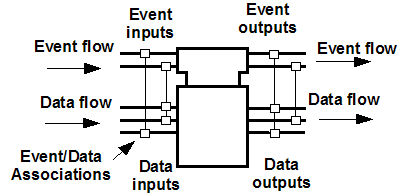
\includegraphics{Figures/IEC61499FunctionBlock}
\decoRule
\caption[IEC 61499 Function Block]{http://www.automation.com/images/isa_automation_week/IEC61499FunctionBlock.png}
\label{fig:IEC61499FunctionBlock}
\end{figure}
 

When comparing IEC 61131-3 and IEC 61499 the biggest difference is in the even-driven execution, while in IEC 61131-3 function was triggered by the cyclic execution.

Cyclic execution was problematic. It does not allow mass using of IEC 61131-3 in distributed systems. This type of execution is 	reliant to the system clock. This approach is not problematic in the scope of one device system. However, in the system with multiple devices there is a problem of sharing the system time. It is practically impossible to run this kind of system synchronously.
In case of the cyclic execution every 1ms and not precise synchronous system it can take up to 1ms to handle any kind of change. In some kind of applications this time delay can lead to the destruction of product, machine or even whole manufacturing system. 
This problem can be solved by decreasing time between two executions. However this solution of delay problem is causing need of bandwidth for data transfer. It leads to the cost of data transport layer increase and also scale up data transfer error rate possibility. 

In IEC 61499 standard this problem was solved by changing cyclic to event driven execution. Function Blocks are not executed cyclically, but are triggered by event. This solution prevents problem with the central time and its sharing and caused also rapid decrease of needed bandwidth. In this approach the data are transferred only when event is triggered. 
For example function block handling the end switch of machine does not have to propagate its state every 1ms like in the previous example. It propagates its state only when change state event occurs. 

There is no support in IEC 61499 for cyclic execution anymore, but for purposes of back compatibility there is a solution of implementing IEC 61131 function into IEC 61499 system. The situation of a program is simply depicted by triggering of the cyclic execution by the use of an E\_CYCLE FB.\cite{4618109} This function block triggers regular event to start execution of IEC 61131-3 compatible applications. 

\section{Types of FB in IEC 61499}

\subsection{Basic FB}
Basic FB (BFB) contains a state machine controlling internal execution called Execution Control Chart (ECC).
ECC consists of three parts: ECC states with associated ECC actions and ECC transitions, which connects the states. ECC transitions are typically guarded by Boolean logical statements. 

When an input event arrives, the first transition with true condition results in state change. With state entry also action associated with this state is executed. Algorithm can access only data input, data output and inner variables. //citovat IEC 61499-1

\begin{figure}[hbp]
\centering
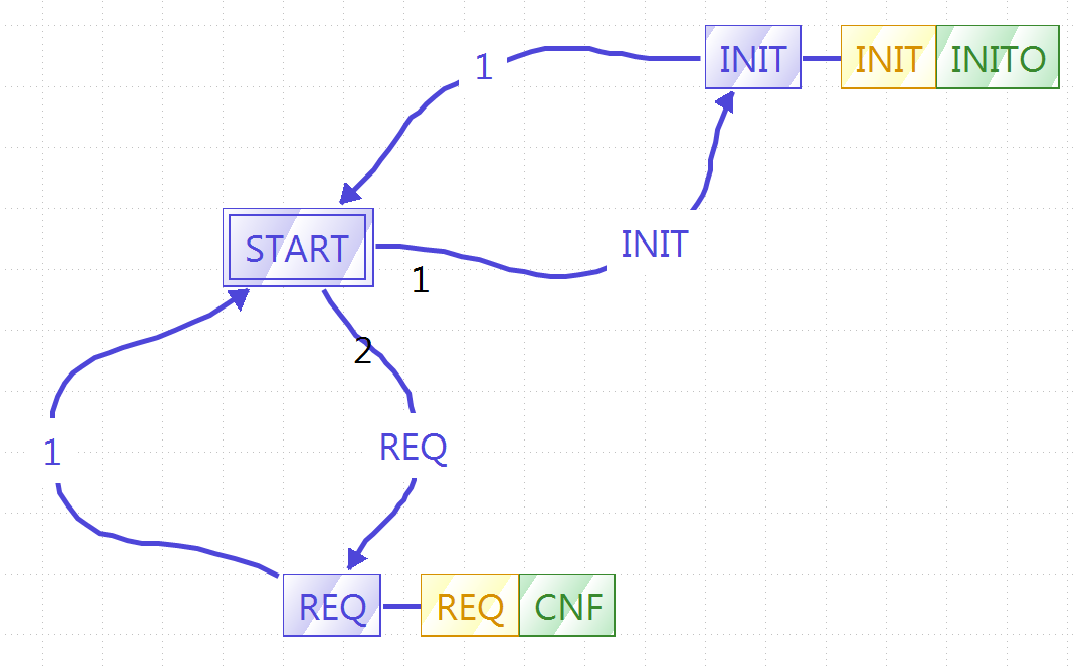
\includegraphics[scale=0.5]{Figures/basicfb-ecc}
\decoRule
\caption[IEC 61499 Basic FB's ECC]{Example of basic FB's ECC}
\label{IEC 61499 Basic FB's ECC}
\end{figure}

\subsection{Composite FB}


Composite FBs (CFBs) are containers for FB dedicated to generate cleaner design. Using Composite FBs developer can create one FB for more complex, many times repeating function consisting of many basic or composite FBs. This allows designer to re-use his design. 
Incomming event and data connections are connected to the internal FBs and also outgoing connections are connected to internal FBs.


\begin{figure}[hbp]
\centering
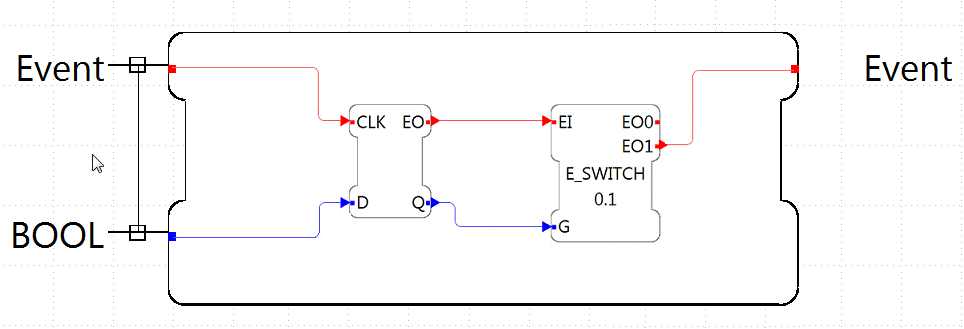
\includegraphics[scale=0.5]{Figures/compositefb}
\decoRule
\caption[IEC 61499 Composite FB]{Example of composite FB structure}
\label{IEC 61499 Composite FB}
\end{figure}

\subsection{Service Interface FB}
Service Interface FB is dedicated to function out of scope of IEC 61499. Typical function is the access to the device's hardware, I/O interface or communication interface. There are two general types of SIFBs in IEC 61499. Requester SIFB and responder SIFB. The requester SIFB remains passive, until it is application-triggered at one of its event inputs. 
The responder type is a resource or hardware triggered FB. It can trigger events by detecting actions of the hardware (e.g. interrupts) without need to trigger this FB from application. 

\section{IEC 61499 Base Model}

Modeling of IEC 61449 system can be divided into two phases. 
In the first phase designer creates Function Block Network by interconnecting of the FBs with data and event connection. In this phase developer has in mind only functionality and it does not depend on any device or control infrastructure. 
In the second phase parts of the system model created in the first phase are mapped to control devices.
For example, in Figure 2.4a, Application 1 is mapped to Devices 2, 3, 4, and 5, whereas Application 2 is mapped only to device 2. 

\begin{figure}[hbp]
\centering
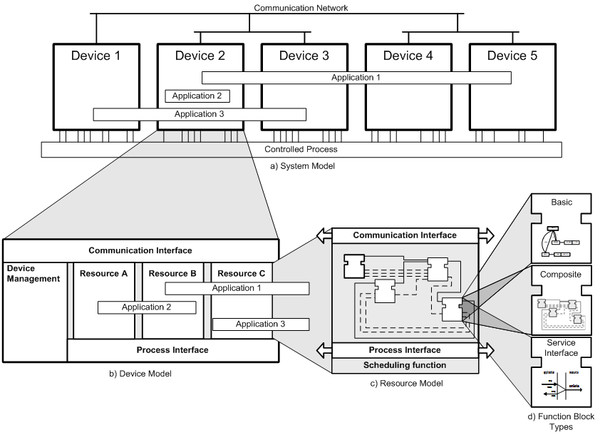
\includegraphics[scale=0.6]{Figures/IEC61499Models}
\decoRule
\caption[IEC 61499 Base Model]{http://2.bp.blogspot.com/-qzJhgeMHSnQ/UNZC7b0op6I/AAAAAAAALwk/aW3FpwY3e5o/s1600/IEC+61499+Models.jpg}
\label{IEC 61499 Base Model}
\end{figure}

IEC 61499 is executed on devices. Every device consist of device management component, communication iterface - provides communication between devices, process interface - provides services for accessing the sensors, actuators and other physical devices needed to control the process. Device can also contain resource. 

Resources are functional units which contain applications or the  parts of applications. Resources in device are independend. This means resources can be added, modified, removed in any particular device without interferring any other resource. This approach is very important to reach the goal of reconfiguration. The task of the resource is to provide execution environment, delivering event notifications.

\section{IEC 61499 applications}
The current application of IEC 61499 can be devided into the research and industrial sector.
IEC 61499 standard exists since January 2005. Before standardization in 2000 it was available in form of so-called Public Available Specification. Although IEC 61499 has been available in some forms for a long time, most published work on the standard up to now has been academic or, if industrially-based has resulted only in prototypical test cases.\cite{4618110}

In industry sector the adoptions of IEC 61499 were mainly case studies and prototypes. A lot of case studies had a starting point via FBDK/FBRT package from Rockwell Automation.
FBRT is implemented in Java and IEC 61499 elements are implemented as Java Classes. This package is a reference implementation and was used to test models and standard. In FBRT the event notification is handeld by function call. The source FB calls notification function of the event connection object and this object triggers event on destination FB by calling his event function. This approach creates delays and is also one of the greatest reasons why FBRT has never been adopted by industry sector. Another reason is also that this Java implementation was not able to run on small industrial control platforms (8/16/32b computers). 


\section{The 4DIAC initiative}

In July 2007 the 4diac open source initiative was founded by PROFACTOR GmbH and the Automation and Control Institute of Vienna University of Technology. 
Nowadays this initiative is conducted with and supported by international automation network O\footnote{3}NEIDA. 


Aim of 4DIAC initiative is to create an open-source framework based on IEC 61499 standard which will provide reference implementation of execution model for IEC 61499.

4DIAC initiative is currently developing two projects IEC 61499 compliant :
\begin{itemize}
	\item 4DIAC IDE - engineering tool
	\item FORTE - runtime environment
\end{itemize}

To work with 4DIAC framework you have to use both of this parts. 

You can find instructions how to install and run this project on your own computer in Appendix A. 
In the next sections brief informations about 4DIAC IDE and FORTE are introduced. These are just the minimal amount of necessary informatios in needs of this thesis.

\section{4DIAC IDE}

4DIAC IDE is IEC 61499 development evironmen based on the Eclipse open tool framework. 
Eclipse base makes 4DIAC IDE multiplatform open source IDE. 

As all other IDEs based on Eclipse work in 4DIAC IDE is divided into perspectives. Every user can create his own perspective, but there are three perspectives which are created by default in 4DIAC IDE. 

This perspective is dedicated to the basic creation of application. FBs can be added, created event and data connection. Below system configuration of one of the example supplied with 4DIAC IDE can be seen. 

Application of figure consist of two devices, connected via Ethernet. Every of this device includes two resources. One of the resources is management resource allways named MGR and read-only.

\begin{figure}[hbp]
\centering
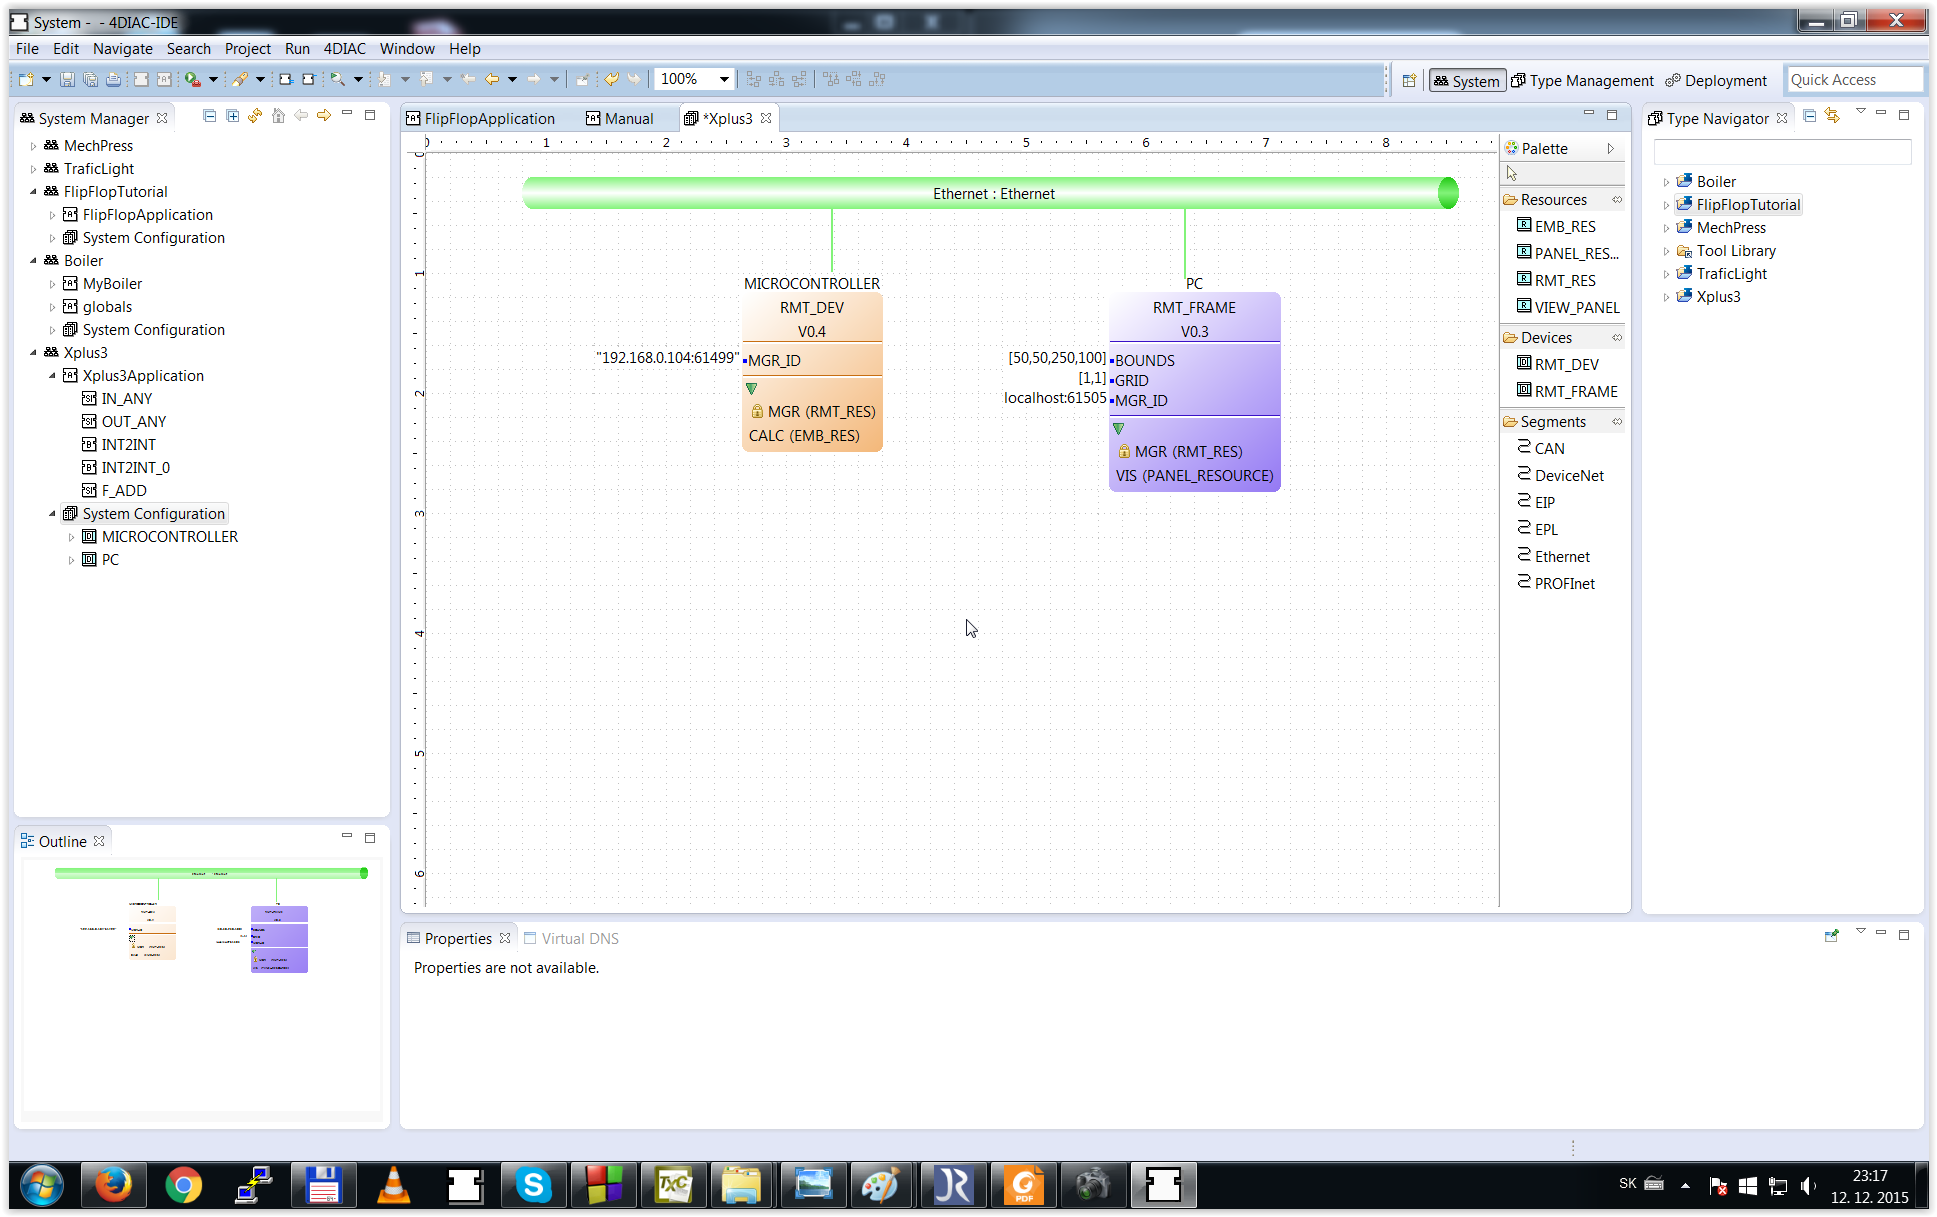
\includegraphics[scale=0.3]{Figures/systemperspective}
\decoRule
\caption[4DIAC IDE System Perspective]{Perspective dedicated to basic creation of application}
\label{4DIAC IDE System Perspective}
\end{figure}

By double clicking on resource you can edit Function Block Network running on this resource.

\begin{figure}[hbp]
\centering
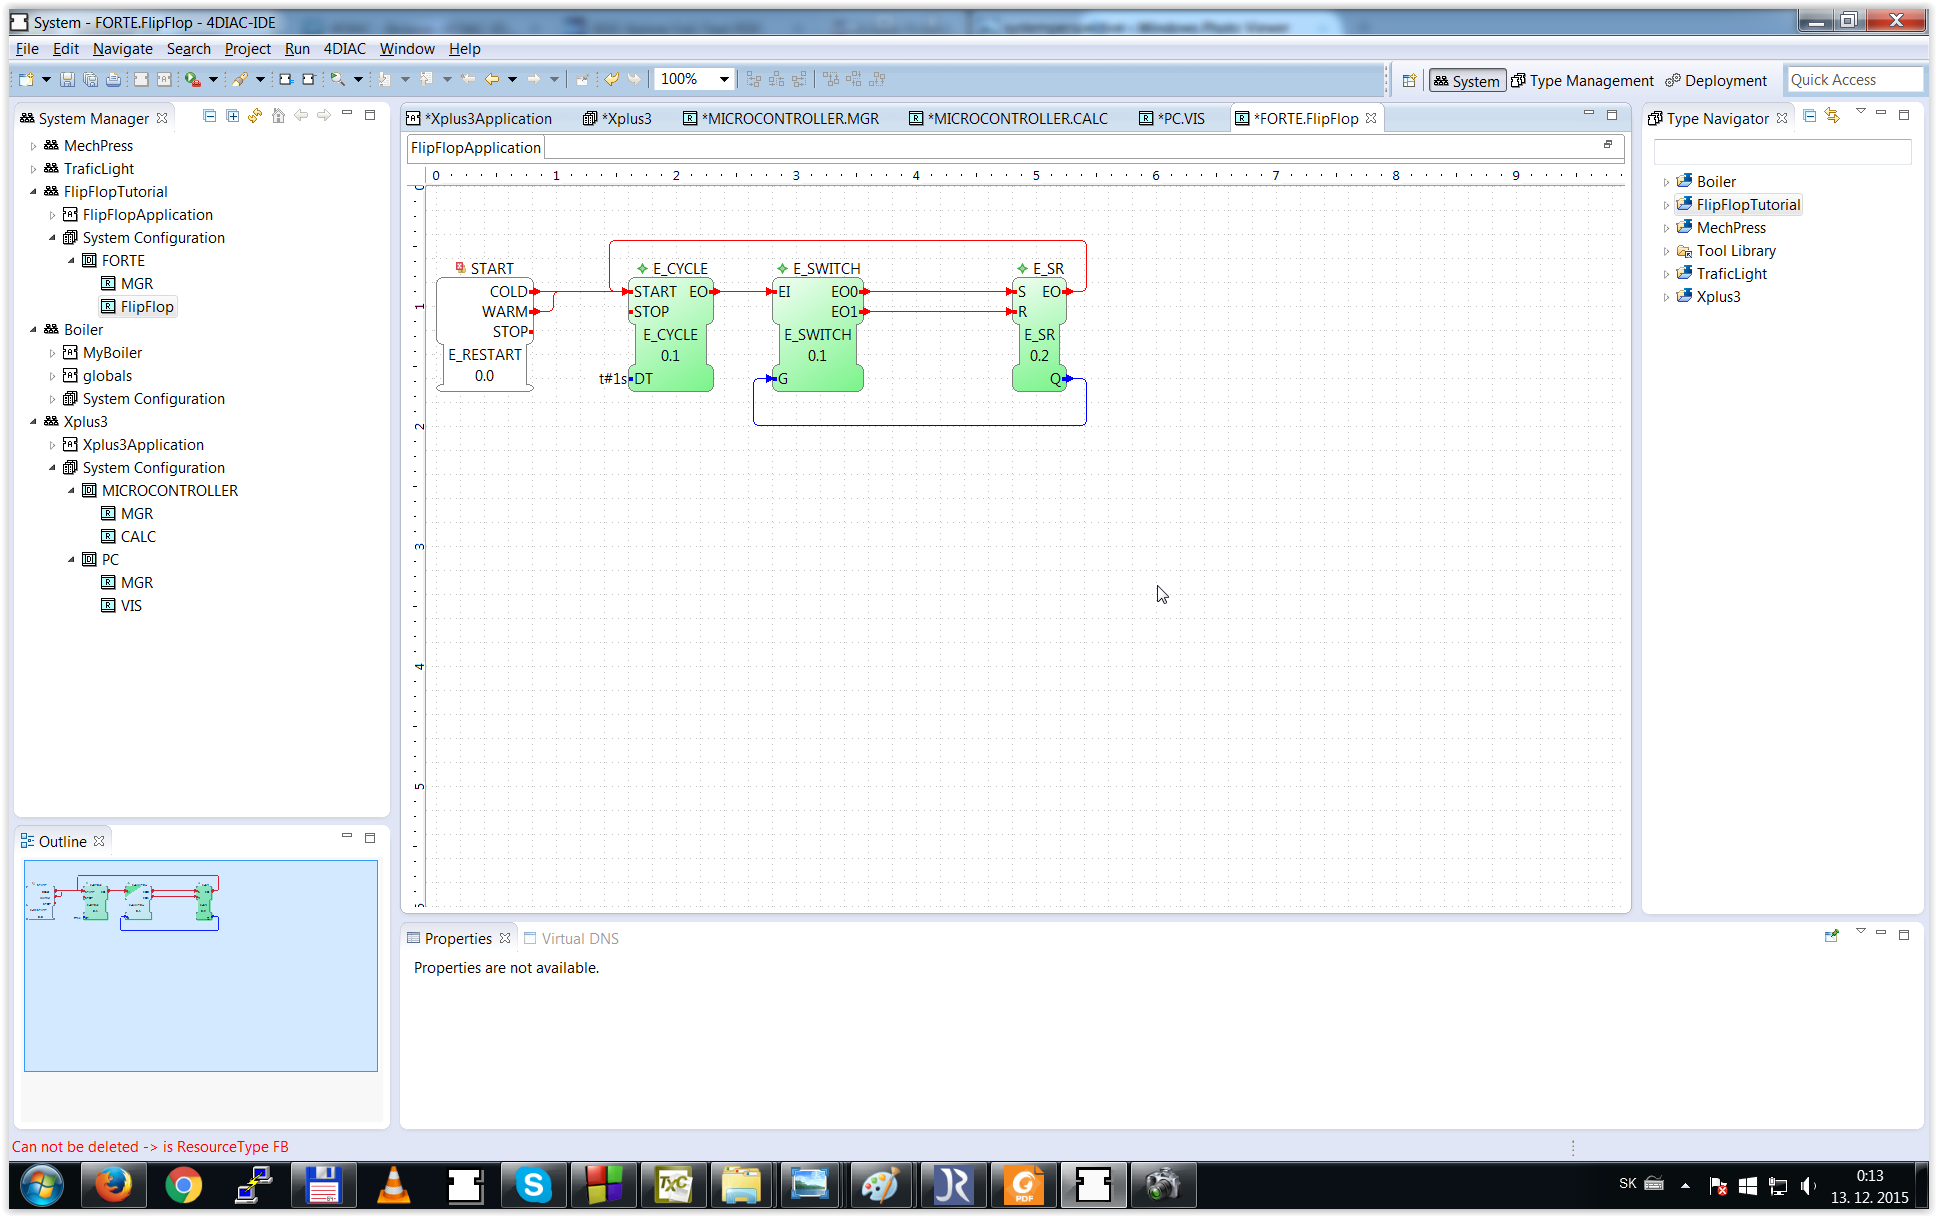
\includegraphics[scale=0.3]{Figures/systemapplicationperspective}
\decoRule
\caption[4DIAC IDE System Perspective - Resource]{Editing Function Block Network in resource}
\label{4DIAC IDE System Perspective - Resource}
\end{figure}

Type Management Perspective is dedicated to editing and creating of developers' own FBs. 
On the figure below, there are shown tools which can be applied on the function block.
In the case of the basic FB you can edit also function of this FB by editing its EEC or Algorithm writen in pseudocode. 
The function of the Composite FB can by modified or created by editing Composite Network. Only Service Interface FBs function is not allowed to change in 4DIAC editor. Function of SIFBs can be modified only by editing forte source. 

All changes made in Type Management Perspective have to be exported into the forte code. To use this modified FBs in control system it is necessary to recompile the FORTE with these updated function block.


\begin{figure}[hbp]
\centering
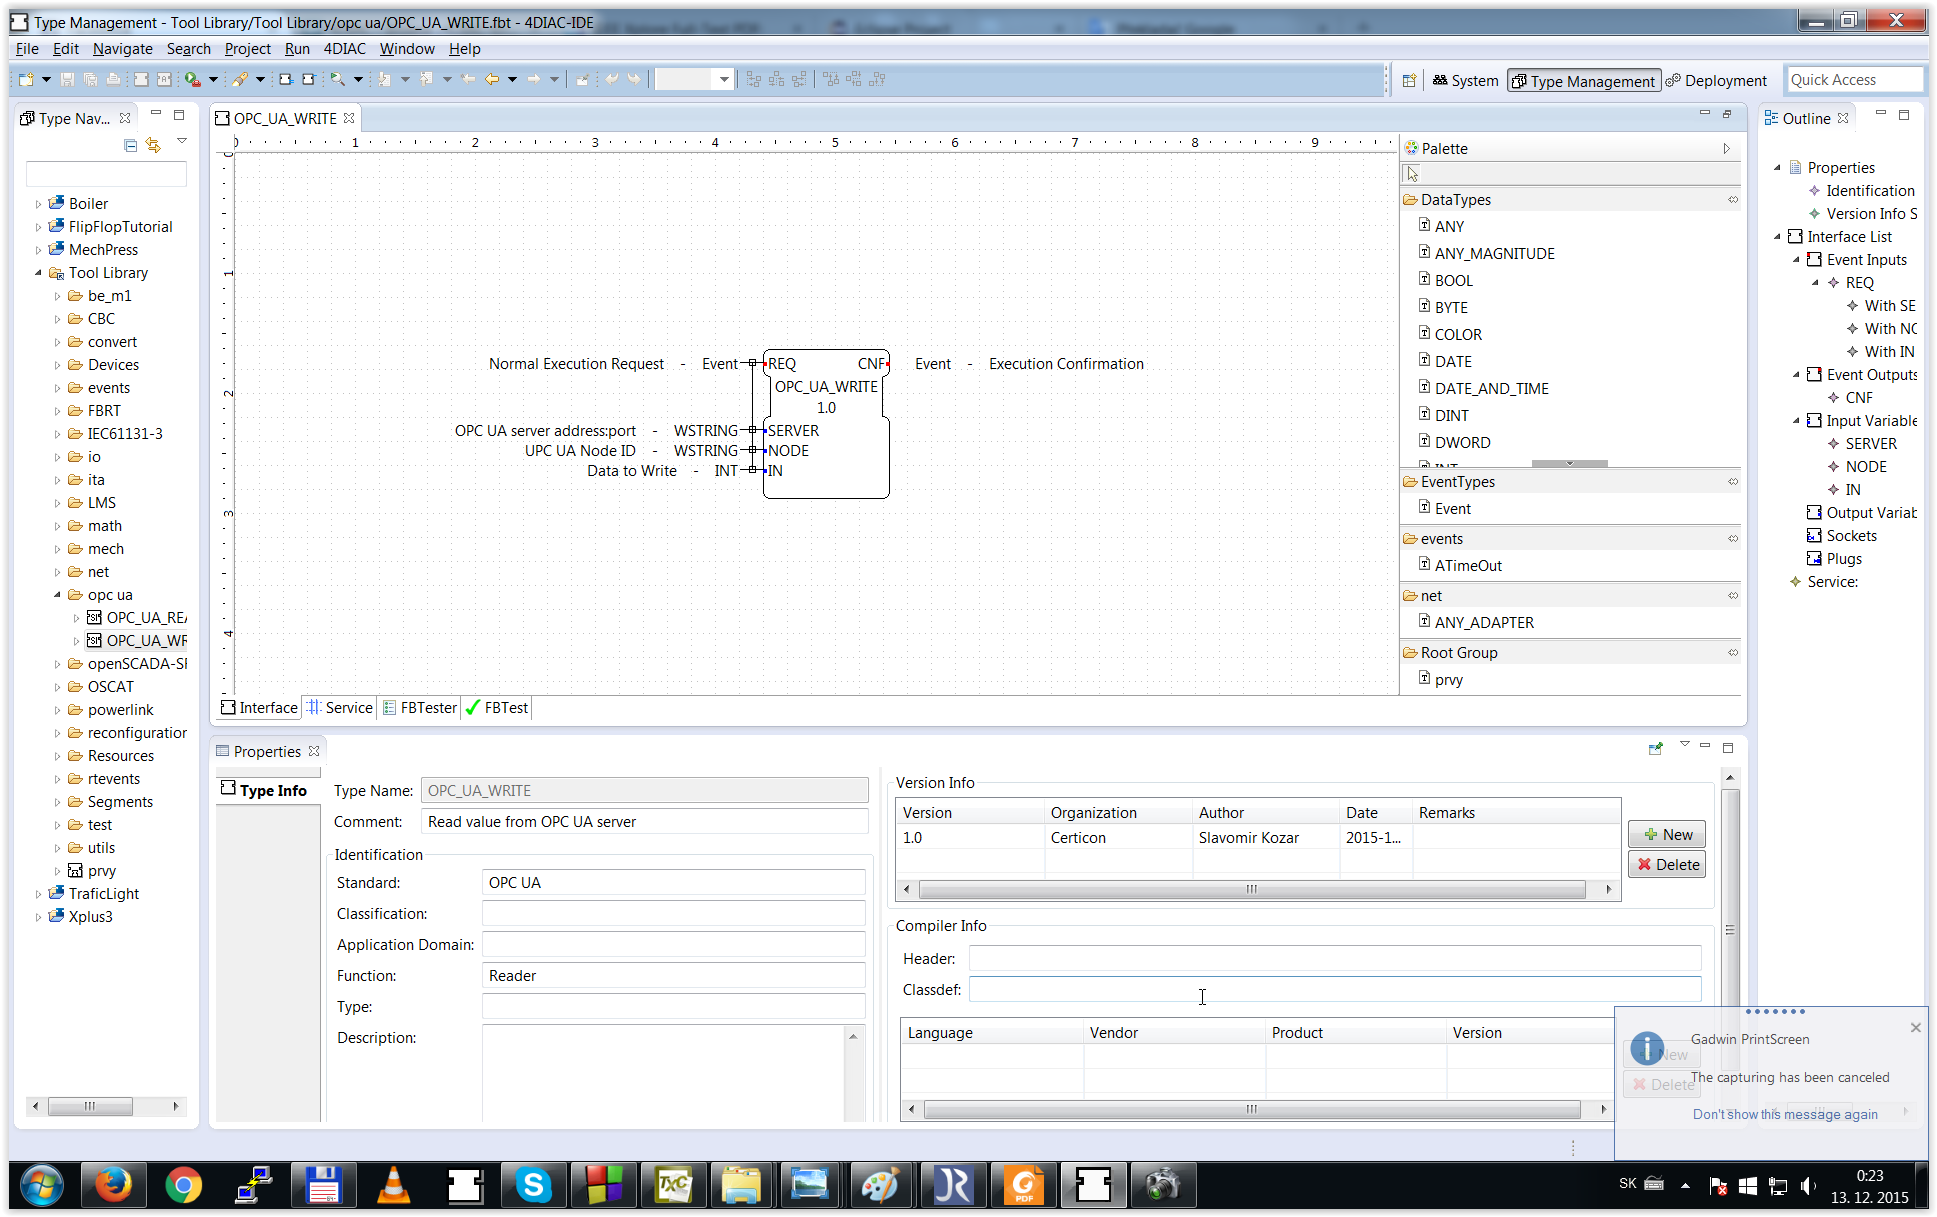
\includegraphics[scale=0.3]{Figures/typemanagementperspective}
\decoRule
\caption[4DIAC IDE Type Management Perspective ]{Editing or Creating FBs}
\label{4DIAC IDE Type Management Perspective}
\end{figure}


Deployment Perspective is dedicated to the deployment and upload application into the control system devices by clicking on Download button.

There is also possibility to run local FORTE and FBRT directly from Deployment Perspective. In case of local FORTE runtime, all its output are shown in Console window. 


\begin{figure}[hbp]
\centering
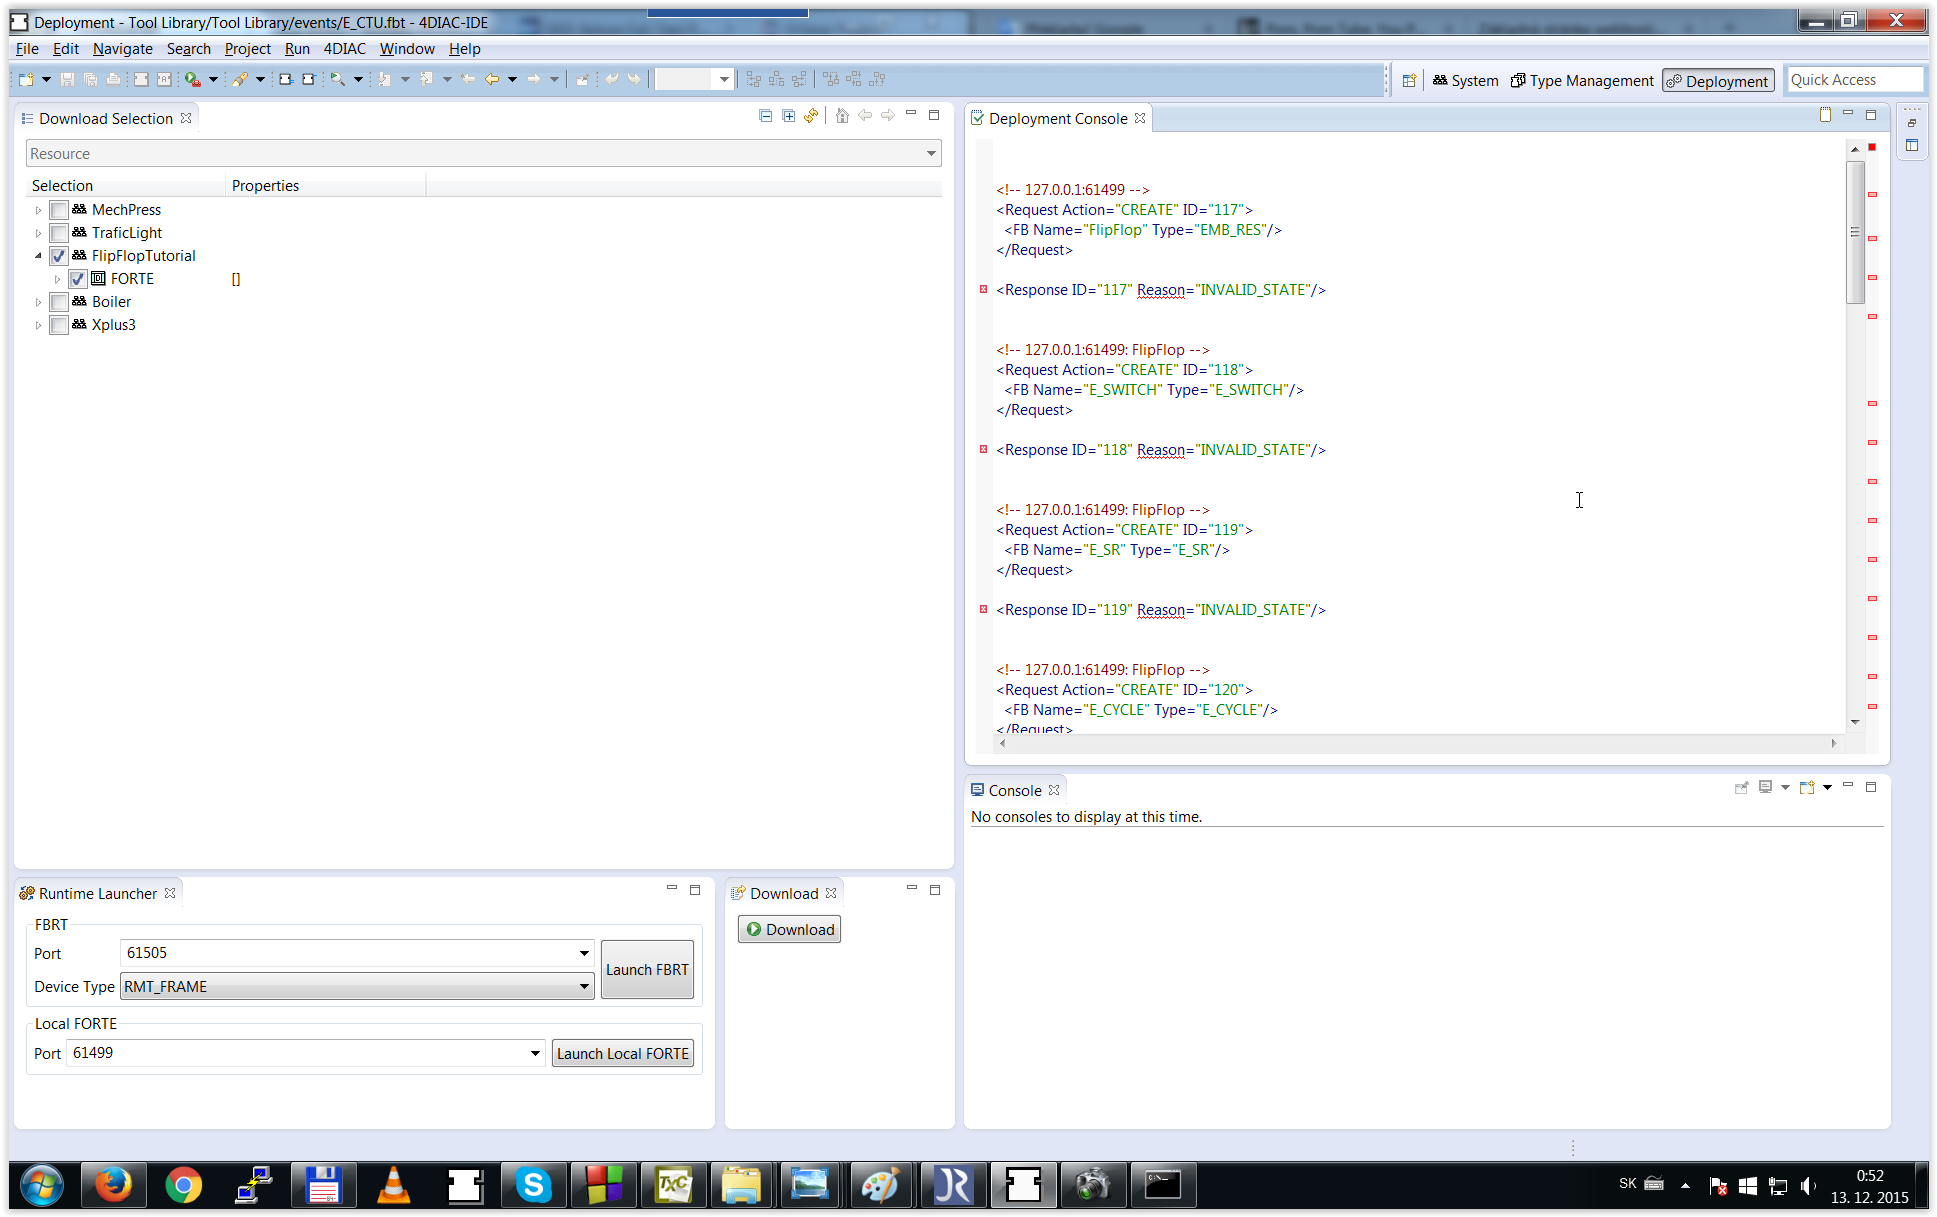
\includegraphics[scale=0.3]{Figures/deploymentperspective}
\decoRule
\caption[4DIAC IDE Deployment Perspective ]{Uploading application into devices}
\label{4DIAC IDE Deployment Perspective}
\end{figure}



\section{4DIAC RUNTIME ENVIRONMENT - FORTE}


The FORTE is a portable C++ implementation of an IEC 61499 runtime environment. It is focused on the small embedded control devices (also 16/ 32 bit controllers) and provides execution of all IEC 61499 types of functions blocks. Currently is forte available for Windows, Posix (Cygwin, Linux), NET+OS 7, eCos. It can be also used on small embedded boards like RaspberryPi, BeagleBone or even Lego Mindstroms nxt. 

\subsection{Function Blocks in the FORTE}
Basic and composite FBs are easy to create and edit in 4DIAC IDE. 
However Service Interfaces FBs, which are most important, because serves connection to the physical devices in control system are defined twice. 
In 4DIAC IDE only outer interface, like event and data inputs outputs are defined function of these function blocks is defined in C++ function generated to every function block. Creating of function block will be discussed in the next chapters. 


